\section{Ticket Generation}
\label{sec:ticket_generation}
For each HR ticket, we create a synthetic employee. Depending on the category of the ticket we want to generate, the employee can have different features. For all tickets' categories, the employees have some common features: \textit{name}, \textit{first name}, \textit{last name}, \textit{nationality}, \textit{country}, \textit{email}, \textit{company}, \textit{company's email} and \textit{ticket date}.\\
All these information are created exploiting the Python library \textit{Faker}\cite{Faraglia_Faker}. The nationality and the company's country are selected from the extendible list \{ USA, Germany, Italy, Spain, France \}. All other information are created accordingly to the country picked. So for example, if the country of birth of the employee is Italy, then the generated name will be Italian. \\
Then, once the employees are generated, the information specific to the ticket category, the ones created starting from the open datasets as mentioned before, are concatenated to the general information of the employees. \\
For each ticket category, there are distinct templates. In each template there is an initial part that contains the general information of the employee, such as name, surname, company\dots, then some prompts correlated to the category of the ticket and then the textual prompt. \\
Here are a couple of examples of templates:\\ \\
Request for time off due to health reasons:
\begin{adjustwidth}{1cm}{}
From: \$\{email\} \\
To: \$\{company email\} \\
First name: \$\{first name\}\\
Last name: \$\{last name\}\\
Company: \$\{company\}\\
Date: \$\{ticket date\}\\
Ticket category: \$\{category\}\\
Ticket sub-category: \$\{sub category\} \\
Date start absence: \$\{date start absence\} \\
Reason absence: \$\{reason\} \\ 
Subject: Request for sick leave for \$\{number of days\} \\ 
\\
Dear Sir/Madame, my name is \$\{name\} and I work at \$\{company\}. I am requesting \textless \textit{generate}\textgreater. I hope \textless \textit{generate}\textgreater. \\ \\

\end{adjustwidth}
Request for refund of travel:
\begin{adjustwidth}{1cm}{}
From: \$\{email\} \\
To: \$\{company email\} \\
First name: \$\{first name\}\\
Last name: \$\{last name\}\\
Company: \$\{company\}\\
Date: \$\{ticket date\}\\
Ticket category: \$\{category\}\\
Ticket sub-category: \$\{sub category\} \\
Date Travel: \$\{date travel\} \\
From: \$\{airport from\}, \$\{from\} \\
Destination: \$\{airport to\}, \$\{to\} \\
Subject: Request of refund for plane ticket from \$\{from\} to \$\{to\} at \$\{date travel\}
\\
Hello, my name is \$\{name\}. I am writing this mail to ask for a refund for the travel \textless \textit{generate}\textgreater \\ \\

\end{adjustwidth}
        
The variables are replaced with the features of the employee, whereas the \textless \textit{generate}\textgreater \space are replaced with text generated by a generative model. The parts generated by the generative model are created recursively. This means that the first \textless generate\textgreater \space is replaced with text generated automatically using as prompt everything that precedes it. Then the second \textless generate\textgreater \space will have as a prompt the entire ticket, including the text generated previously by the model. The model is forced to generate some text, if no text is generated in an iteration, the process is repeated until the model gives a non-empty output. \\
A general schema of the generation is shown in \autoref{fig:schema_topic_generation}

\begin{figure}[h] 
    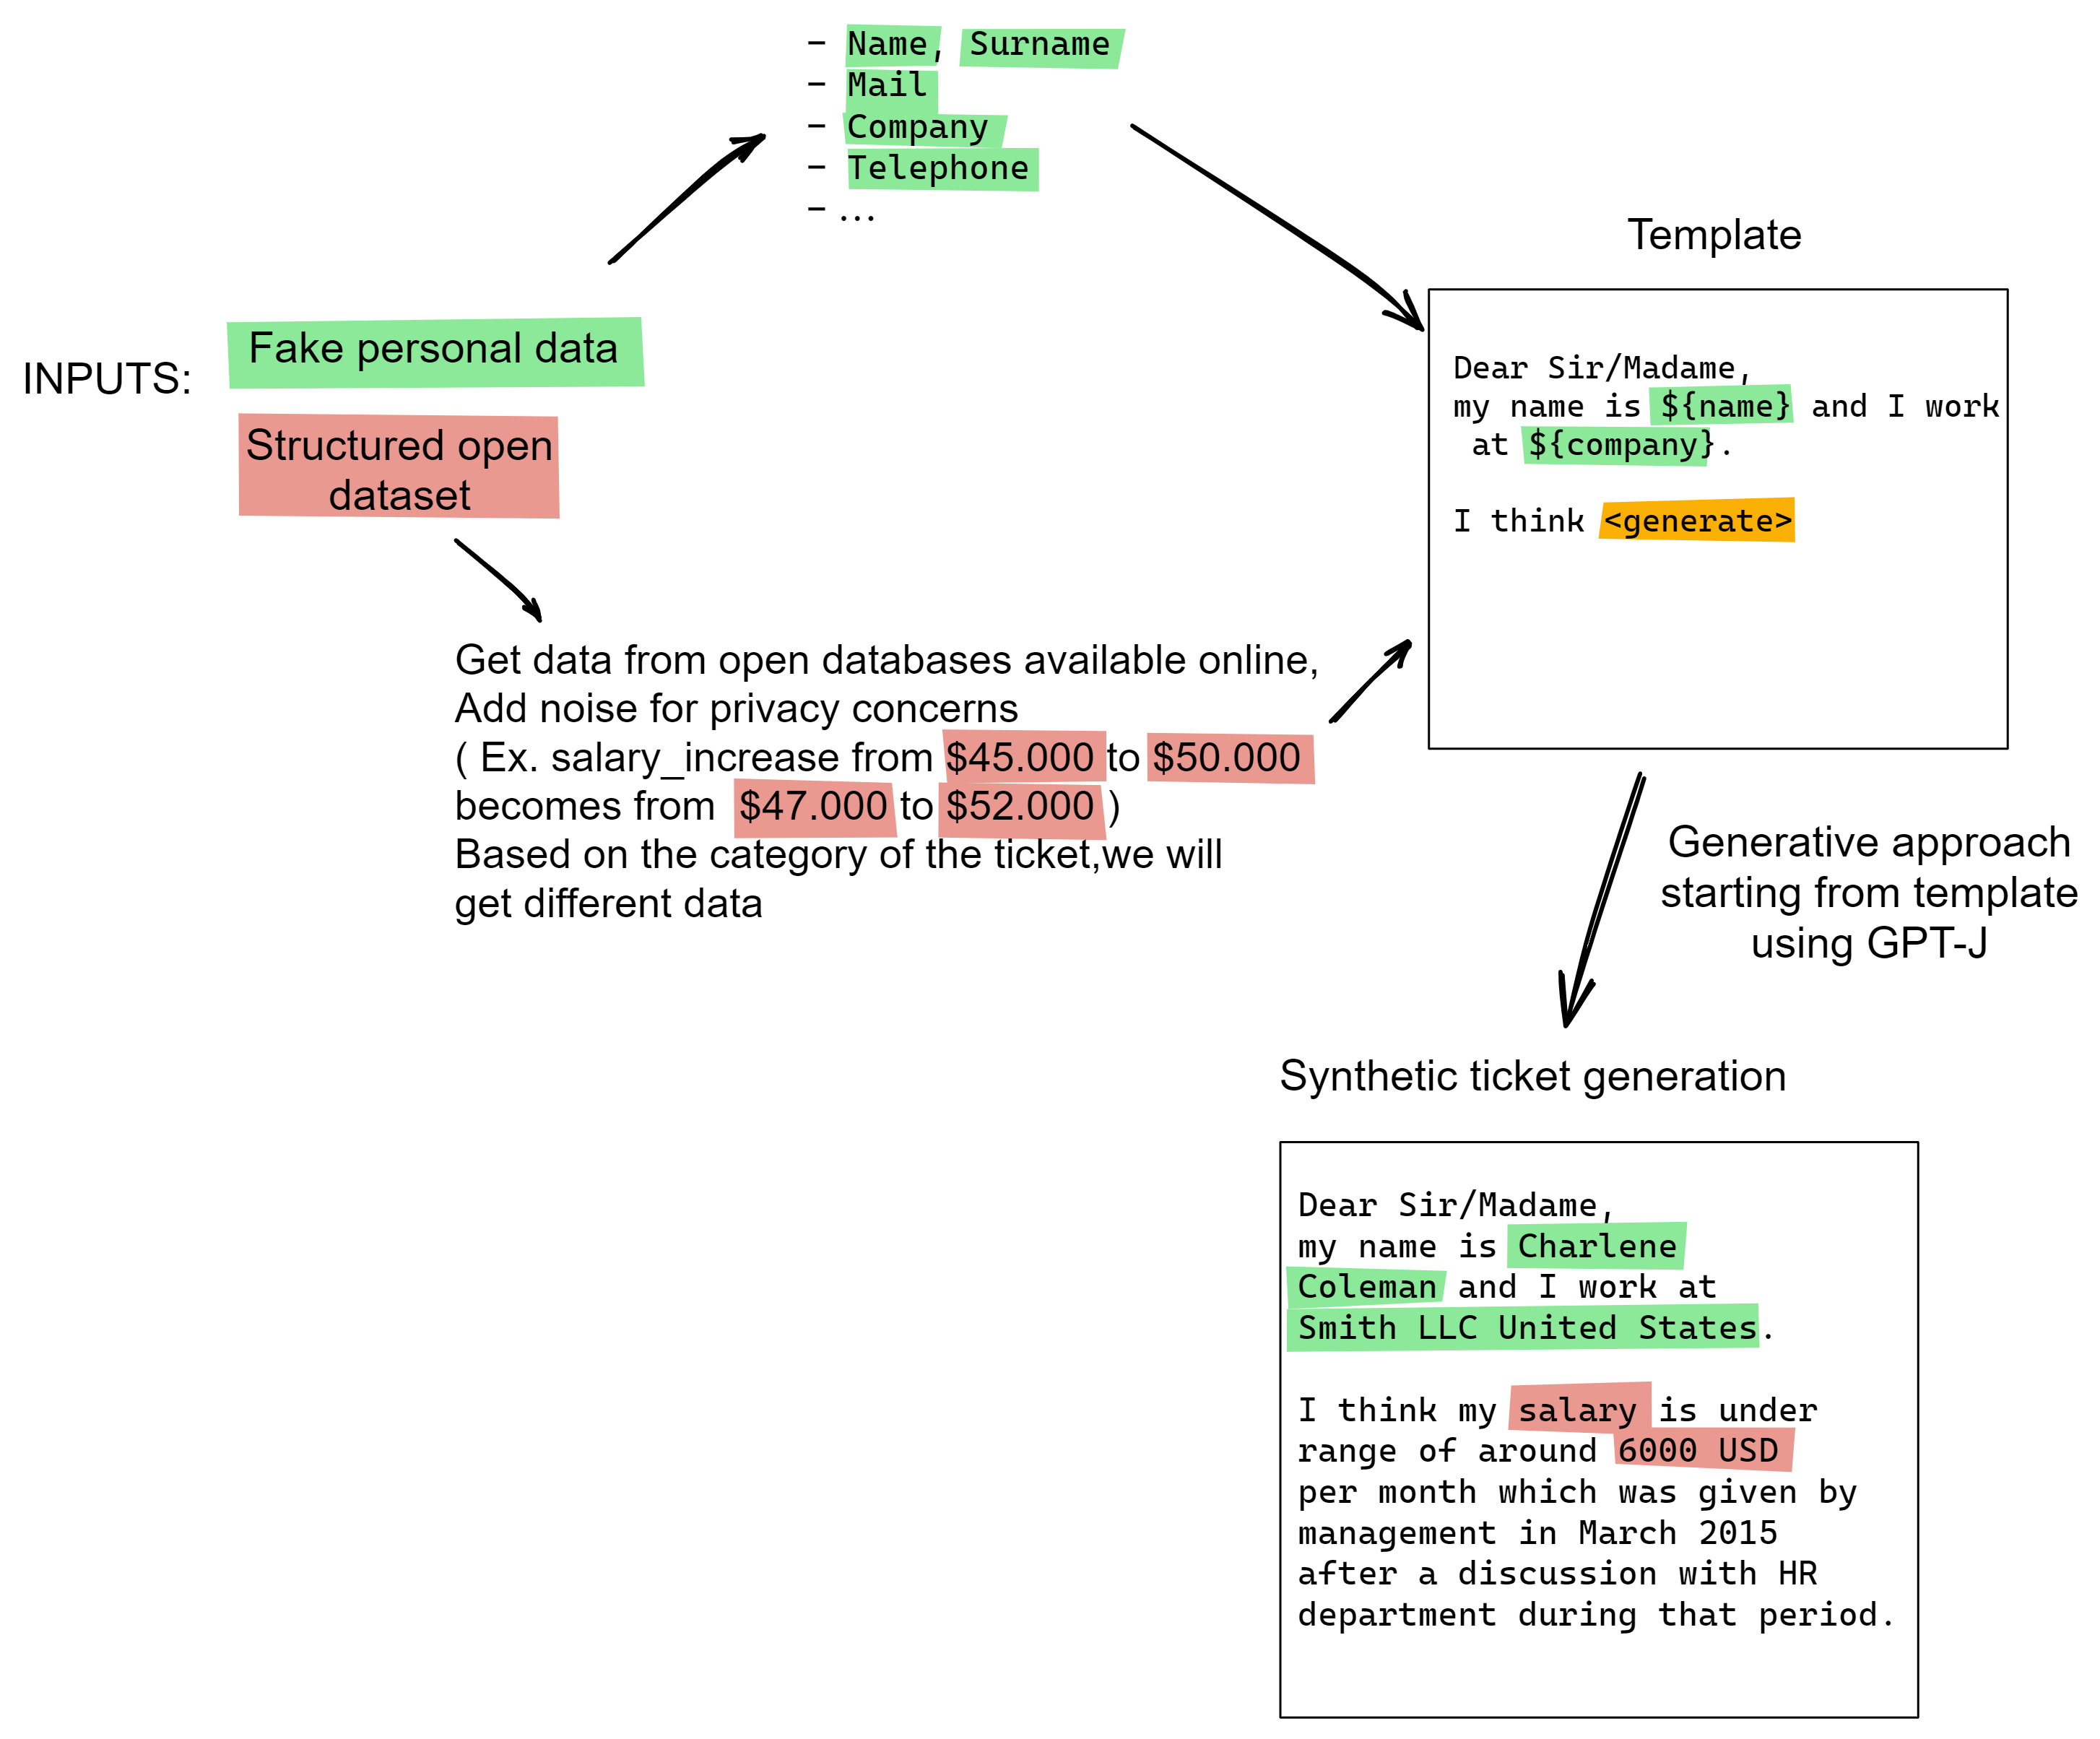
\includegraphics[width=\textwidth]{images/ticket_creation_schema.png}
    \caption{Schema of Ticket Generation}
    \label{fig:schema_topic_generation}
\end{figure}    


\subsection*{Templates}
\label{sec:templates}
Generative Pre-trained Transformer (GPT)\todo{added the acronym here} \cite{radford2018improving} models take in a prompt, or context, and generate text from it. The prompts typically take the form of a few sentences or a paragraph, and the models generate sentences that fit the context of the prompt. By manipulating the prompt, users can generate text of various tones, topics, and styles. \\
The GPT models are also capable of completing tasks such as question answering, machine translation, and summarization in an unsupervised manner\cite{radford2019language}. By providing a prompt with the task and context, the models can generate accurate results that address the specific context and task. For example, summarization tasks require a prompt to provide the necessary data so that the model can deliver a correct summary of the text. \\
Changing the prompt of GPT can change the tone, topics, and style of the generated text. Depending on the prompt, GPT models can generate text ranging from creative stories to technical summaries. The tone and style of the text can range from humorous to academic, depending on the prompt. As the prompt changes, the model will also adjust to reflect the context of the prompt. \\
This is why we took inspiration from the e-mail format, as HR tickets are created in a working environment where formal language is used and often they resemble emails in the tone and the topics. \\
The emails of the \textit{Enron dataset}, one of the few datasets of emails public available, have usually a well-structured prompt, here's an example: 
\begin{adjustwidth}{1cm}{}
    Message-ID: <16593073.1075858228177.JavaMail.evans@thyme>\\
    Date: Wed, 12 Jan 2000 00:29:00 -0800 (PST) \\
    From: carrie.hollomon@enron.com\\
    To: phillip.love@enron.com\\
    Subject: Workhours\\
    Mime-Version: 1.0\\
    Content-Type: text/plain; charset=us-ascii\\
    Content-Transfer-Encoding: 7bit\\\\
    Hello \dots
\end{adjustwidth}
To mimic the format of the emails of the \textit{Enron dataset}, we kept the From, To, Date and Subject rows. Instead, we removed the Mime-Version, the Content-type and Content-Transfer-Encoding, because after conducting some experiments it was evident that they did not help to achieve better results, on the contrary in some cases they were worse. \\
In addition to the standard information, we added some rows with additional information specific to the category, rather than including them only in the subject or in the initial prompt. \\
\\
In order to generate tickets that were dissimilar and covered a wide range of topics/tokens, we preferred giving GPT small text prompts and letting the model generate most of the text getting the information from the email-like prompt. This approach allowed us to improve the diversity of the dataset and, consequently, its usefulness. \\
\\
Small text prompt example of a request for shift change:
\begin{adjustwidth}{1cm}{}
    Dear Sir/Madame, my name is \$\{name\}. I wanted to \textless \textit{generate}\textgreater
\end{adjustwidth}

Long text prompt example of a request for shift change:
\begin{adjustwidth}{1cm}{}
    Dear Sir/Madame, my name is \$\{name\} and I work at \$\{company\}. I wanted to ask to change the shift from \$\{old\_date\} to \$\{new\_date\} in order to be able to \textless \textit{generate} \textgreater
\end{adjustwidth}